%% BioMed_Central_Tex_Template_v1.06
%%                                      %
%  bmc_article.tex            ver: 1.06 %
%                                       %

%%IMPORTANT: do not delete the first line of this template
%%It must be present to enable the BMC Submission system to
%%recognise this template!!

%%%%%%%%%%%%%%%%%%%%%%%%%%%%%%%%%%%%%%%%%
%%                                     %%
%%  LaTeX template for BioMed Central  %%
%%     journal article submissions     %%
%%                                     %%
%%          <8 June 2012>              %%
%%                                     %%
%%                                     %%
%%%%%%%%%%%%%%%%%%%%%%%%%%%%%%%%%%%%%%%%%


%%%%%%%%%%%%%%%%%%%%%%%%%%%%%%%%%%%%%%%%%%%%%%%%%%%%%%%%%%%%%%%%%%%%%
%%                                                                 %%
%% For instructions on how to fill out this Tex template           %%
%% document please refer to Readme.html and the instructions for   %%
%% authors page on the biomed central website                      %%
%% http://www.biomedcentral.com/info/authors/                      %%
%%                                                                 %%
%% Please do not use \input{...} to include other tex files.       %%
%% Submit your LaTeX manuscript as one .tex document.              %%
%%                                                                 %%
%% All additional figures and files should be attached             %%
%% separately and not embedded in the \TeX\ document itself.       %%
%%                                                                 %%
%% BioMed Central currently use the MikTex distribution of         %%
%% TeX for Windows) of TeX and LaTeX.  This is available from      %%
%% http://www.miktex.org                                           %%
%%                                                                 %%
%%%%%%%%%%%%%%%%%%%%%%%%%%%%%%%%%%%%%%%%%%%%%%%%%%%%%%%%%%%%%%%%%%%%%

%%% additional documentclass options:
%  [doublespacing]
%  [linenumbers]   - put the line numbers on margins

%%% loading packages, author definitions

%\documentclass[twocolumn]{bmcart}% uncomment this for twocolumn layout and comment line below
\documentclass{bmcart}

%%% Load packages
%\usepackage{amsthm,amsmath}
%\RequirePackage{natbib}
%\RequirePackage[authoryear]{natbib}% uncomment this for author-year bibliography
%\RequirePackage{hyperref}
\usepackage[utf8]{inputenc} %unicode support
%\usepackage[applemac]{inputenc} %applemac support if unicode package fails
%\usepackage[latin1]{inputenc} %UNIX support if unicode package fails
\usepackage{graphicx}
\usepackage{booktabs}
\usepackage{amsfonts}
\usepackage{subfig}
\usepackage[ruled,lined]{algorithm2e}
\usepackage{multirow}
\usepackage{color}
\usepackage{flushend}
\usepackage[bookmarks=false]{hyperref}
\usepackage{setspace} % for setstretch in algorithm
\usepackage{amssymb, amsmath}
\usepackage{xspace}


%%%%%%%%%%%%%%%%%%%%%%%%%%%%%%%%%%%%%%%%%%%%%%%%%
%%                                             %%
%%  If you wish to display your graphics for   %%
%%  your own use using includegraphic or       %%
%%  includegraphics, then comment out the      %%
%%  following two lines of code.               %%
%%  NB: These line *must* be included when     %%
%%  submitting to BMC.                         %%
%%  All figure files must be submitted as      %%
%%  separate graphics through the BMC          %%
%%  submission process, not included in the    %%
%%  submitted article.                         %%
%%                                             %%
%%%%%%%%%%%%%%%%%%%%%%%%%%%%%%%%%%%%%%%%%%%%%%%%%


%%% Put your definitions there:
\startlocaldefs
\endlocaldefs

\newcommand{\red}[1]{\textcolor{red}{#1}}
\newcommand{\tylde}{$\sim$}

%\hypersetup{colorlinks=true,linkcolor=black,citecolor=black}

\SetKwInput{KwData}{Global params.}

\def\qrand{q_{rand}}
\def\qstart{q_{start}}
\def\qinit{\qstart}
\def\qgoal{q_{goal}}
\def\qnear{q_{near}}
\def\qnew{q_{new}}
\def\T{\mathcal{T}}

\def\C{\mathcal{C}}
\def\CF{\mathcal{C}_{free}}
\def\dtg{d_{t}}
\def\dist{\varrho}
\def\distt{\varrho_{3D}}
\def\R{\mathbb{R}}

%\def\rv{R_{tunnel}}


\def\Imax{I_{max}} %max number of iterations of RRT-based planners

\SetKw{return}{return}

\def\sdelta{s_{\Delta}}


\def\probe{r_{\mathrm{probe}}}
\def\Sprobe{S_{\mathrm{probe}}}

\def\gprobe{r_{\mathrm{out}}}
\def\Sgprobe{S_{\mathrm{out}}}


\def\CG{\mathcal{C}_{goal}}
\def\SB{\mathbf{S}_{blocking}}
\def\SS{\mathbf{S}}


%spacing for algorithm environment. 1.0 mean normal spacing
\def\gb{p_{tunnel}}

\def\L{\mathcal{L}}
\def\S{\mathcal{S}}

\def\LA{L_1}
\def\LB{L_2}

\def\RA{A$_{1}$}
\def\RB{A$_{2}$}
\def\RC{A$_{1}^{*}$}
\def\RD{A$_1^P$}

%%% Begin ...
\begin{document}

%%% Start of article front matter
\begin{frontmatter}

\begin{fmbox}
\dochead{Research}

%%%%%%%%%%%%%%%%%%%%%%%%%%%%%%%%%%%%%%%%%%%%%%
%%                                          %%
%% Enter the title of your article here     %%
%%                                          %%
%%%%%%%%%%%%%%%%%%%%%%%%%%%%%%%%%%%%%%%%%%%%%%

\title{Motion Planning for Assessing the Accessibility of Protein Tunnels}

%%%%%%%%%%%%%%%%%%%%%%%%%%%%%%%%%%%%%%%%%%%%%%
%%                                          %%
%% Enter the authors here                   %%
%%                                          %%
%% Specify information, if available,       %%
%% in the form:                             %%
%%   <key>={<id1>,<id2>}                    %%
%%   <key>=                                 %%
%% Comment or delete the keys which are     %%
%% not used. Repeat \author command as much %%
%% as required.                             %%
%%                                          %%
%%%%%%%%%%%%%%%%%%%%%%%%%%%%%%%%%%%%%%%%%%%%%%

\author[
   addressref={aff1},                   % id's of addresses, e.g. {aff1,aff2}
   corref={aff1},                       % id of corresponding address, if any
  % noteref={n1},                        % id's of article notes, if any
   email={vonasek@labe.felk.cvut.cz}   % email address
]{\inits{VV}\fnm{Vojt\v ech} \snm{Von\' asek}}
\author[
   addressref={aff2},
   %email={john.RS.Smith@cambridge.co.uk}
]{\inits{BK}\fnm{Barbora} \snm{Kozl\'\i kov\'a}}
\author[
   addressref={aff2},
   %email={john.RS.Smith@cambridge.co.uk}
]{\inits{AJ}\fnm{Adam} \snm{Jur\v{c}\'\i k}}
\author[
   addressref={aff3,aff4},
]{\inits{OV}\fnm{Ond\v{r}ej} \snm{V\'{a}vra}}
\author[
   addressref={aff1},
   %email={john.RS.Smith@cambridge.co.uk}
]{\inits{MS}\fnm{Martin} \snm{Saska}}


%%%%%%%%%%%%%%%%%%%%%%%%%%%%%%%%%%%%%%%%%%%%%%
%%                                          %%
%% Enter the authors' addresses here        %%
%%                                          %%
%% Repeat \address commands as much as      %%
%% required.                                %%
%%                                          %%
%%%%%%%%%%%%%%%%%%%%%%%%%%%%%%%%%%%%%%%%%%%%%%

\address[id=aff1]{%                           % unique id
  \orgname{Faculty of Electrical Engineering,  Czech Technical University in Prague}, % university, etc
  \street{Technick\'a 2},                     %
  %\postcode{}                                % post or zip code
  \city{Prague},                              % city
  \cny{Czech Republic}                                    % country
}
\address[id=aff2]{%
  \orgname{Faculty of Informatics, Masaryk University},
  \street{Botanick\'a 68a},
  %\postcode{24105}
  \city{Brno},
  \cny{Czech Republic}
}
\address[id=aff3]{%
  \orgname{Loschmidt Laboratories, Department of Experimental Biology RECETOX, Faculty of Science, Masaryk University},
  \street{Kamenice 5},
  %\postcode{24105}
  \city{Brno},
  \cny{Czech Republic}
}
\address[id=aff4]{%
  \orgname{International Centre for Clinical Research, St. Anne’s University Hospital},
  %  Brno, Pekařská 53, 656 91 Brno, Czech Republic
  \street{Peka\v{r}sk\'a 53}
  \city{Brno},
  \cny{Czech Republic}
}


%%%%%%%%%%%%%%%%%%%%%%%%%%%%%%%%%%%%%%%%%%%%%%
%%                                          %%
%% Enter short notes here                   %%
%%                                          %%
%% Short notes will be after addresses      %%
%% on first page.                           %%
%%                                          %%
%%%%%%%%%%%%%%%%%%%%%%%%%%%%%%%%%%%%%%%%%%%%%%

%\begin{artnotes}
%\note{Sample of title note}     % note to the article
%\note[id=n1]{Equal contributor} % note, connected to author
%\end{artnotes}

\end{fmbox}% comment this for two column layout

%%%%%%%%%%%%%%%%%%%%%%%%%%%%%%%%%%%%%%%%%%%%%%
%%                                          %%
%% The Abstract begins here                 %%
%%                                          %%
%% Please refer to the Instructions for     %%
%% authors on http://www.biomedcentral.com  %%
%% and include the section headings         %%
%% accordingly for your article type.       %%
%%                                          %%
%%%%%%%%%%%%%%%%%%%%%%%%%%%%%%%%%%%%%%%%%%%%%%

{\color{red}revise authors}

\begin{abstractbox}

\begin{abstract} % abstract
\parttitle{Background} %if any
Chemical interactions between proteins and other molecules (ligands) take place in specific locations, called active sites, that are often deeply buried inside the protein structure.
These active sites are accessible through one or more void paths, called tunnels.
Nowadays, tunnels are mostly computed using Voronoi diagrams which approximate the ligand by a bounding sphere and 
the traversability of the tunnels is determined based only on the radial bottlenecks.
This can lead to imprecise results as the shape of the ligand is not considered.

\parttitle{Results} %if any
We propose an alternative method to compute trajectories of ligands along selected tunnels in the proteins.
The trajectories are computed using a novel motion planner, based on Rapidly Exploring Random Tress, that searches
the corresponding configuration space, determined by the Voronoi-based tunnel.
In our approach, the flexibility of the ligand is modeled by allowing the rotations in its dihedral angles.
The search of the trajectories is guided using the information about a tunnel (its spherical representation), calculated using Voronoi diagrams.
By constraining the search to the vicinity of such a tunnel, the ligand trajectories can be found significantly faster than when using other dedicated tools.
The resulted trajectories can be further evaluated wrt. their biochemical relevance by calculating the energy  profile, which enables the biochemists to decide if the analyzed tunnel is feasible for accessing the given ligand.

\parttitle{Conclusions} %if any
The proposed method has been evaluated using a virtual screening scenario to estimate the traversability of tunnels for several ligands. The results are summarized in a set of performance tables.
\end{abstract}

%%%%%%%%%%%%%%%%%%%%%%%%%%%%%%%%%%%%%%%%%%%%%%
%%                                          %%
%% The keywords begin here                  %%
%%                                          %%
%% Put each keyword in separate \kwd{}.     %%
%%                                          %%
%%%%%%%%%%%%%%%%%%%%%%%%%%%%%%%%%%%%%%%%%%%%%%

\begin{keyword}
\kwd{protein}
\kwd{tunnel}
\kwd{motion planning}
\end{keyword}

% MSC classifications codes, if any
%\begin{keyword}[class=AMS]
%\kwd[Primary ]{}
%\kwd{}
%\kwd[; secondary ]{}
%\end{keyword}

\end{abstractbox}
%
%\end{fmbox}% uncomment this for twcolumn layout

\end{frontmatter}

%%%%%%%%%%%%%%%%%%%%%%%%%%%%%%%%%%%%%%%%%%%%%%
%%                                          %%
%% The Main Body begins here                %%
%%                                          %%
%% Please refer to the instructions for     %%
%% authors on:                              %%
%% http://www.biomedcentral.com/info/authors%%
%% and include the section headings         %%
%% accordingly for your article type.       %%
%%                                          %%
%% See the Results and Discussion section   %%
%% for details on how to create sub-sections%%
%%                                          %%
%% use \cite{...} to cite references        %%
%%  \cite{koon} and                         %%
%%  \cite{oreg,khar,zvai,xjon,schn,pond}    %%
%%  \nocite{smith,marg,hunn,advi,koha,mouse}%%
%%                                          %%
%%%%%%%%%%%%%%%%%%%%%%%%%%%%%%%%%%%%%%%%%%%%%%

%%%%%%%%%%%%%%%%%%%%%%%%% start of article main body
% <put your article body there>

%%%%%%%%%%%%%%%%
%% Background %%
%%
\section*{Background}

Reactivity of proteins with other molecules plays a crucial role in many research disciplines, including protein engineering and drug design.
Protein reactivity is tightly connected with the presence of the void space in its inner structure.
This void space can be categorized according to its position and accessibility from the protein surface. 
As many chemical reactions are undergoing deeply inside the protein structure, it is crucial to be able to transport a small molecule (ligand) to this inner area.
For this purpose, the molecule uses a void space, connecting this inner area (active site) with the protein surface.
This space, forming a void path inside the protein structure, is denoted as a tunnel.
Ligands entering the active site via these tunnels can the react with the amino acids surrounding the active site~\cite{gora2013gates,marques2017enzyme} (see Fig.~\ref{fig::motiv}) and the product of such a reaction can serve as a basis of new medication or can control and influence the protein properties. 
 
%This space, forming a path called tunnel, can be utilized by a small molecule (ligand) which can enter the protein inner space and react with the amino acids surrounding the protein active site~\cite{gora2013gates,marques2017enzyme} (see Fig.~\ref{fig::motiv}).
The location and size of the tunnel determine the size and shape of a ligand passing through this tunnel to the active site.
Currently, the biochemists can use various computational methods for tunnel detection in order to estimate the possibility of interactions between the protein and ligand.
The ultimate goal of all these methods is to reduce the number of necessary in-vitro experiments.

Protein properties and its reactivity are influenced not only by its constitution, but also its dynamic behavior in real environment plays a crucial role~\cite{zhou2010gates,dynasome}.
Therefore, some of the existing methods enable to detect and track tunnels in the molecular dynamics simulations as well. 
Here, the tunnel stability over time is a crucial additional parameter influencing the tunnel biochemical relevance. 


The most common tools detect the tunnels by using Voronoi diagrams~\cite{yaffe2008,caver3}, assuming a spherical ligand (probe), 
i.e., they approximate the ligand by a bounding sphere.
However, ligands are typically of non-spherical shape, which is completely ignored by these methods. 
%This can lead to very imprecise result, especially for elongated ligands, as the feasible tunnels can be completely omitted.

\begin{figure}[t]
\centering
{\footnotesize
\renewcommand{\arraystretch}{-0.5}
\renewcommand{\tabcolsep}{-1pt}
\begin{tabular}{ccc}
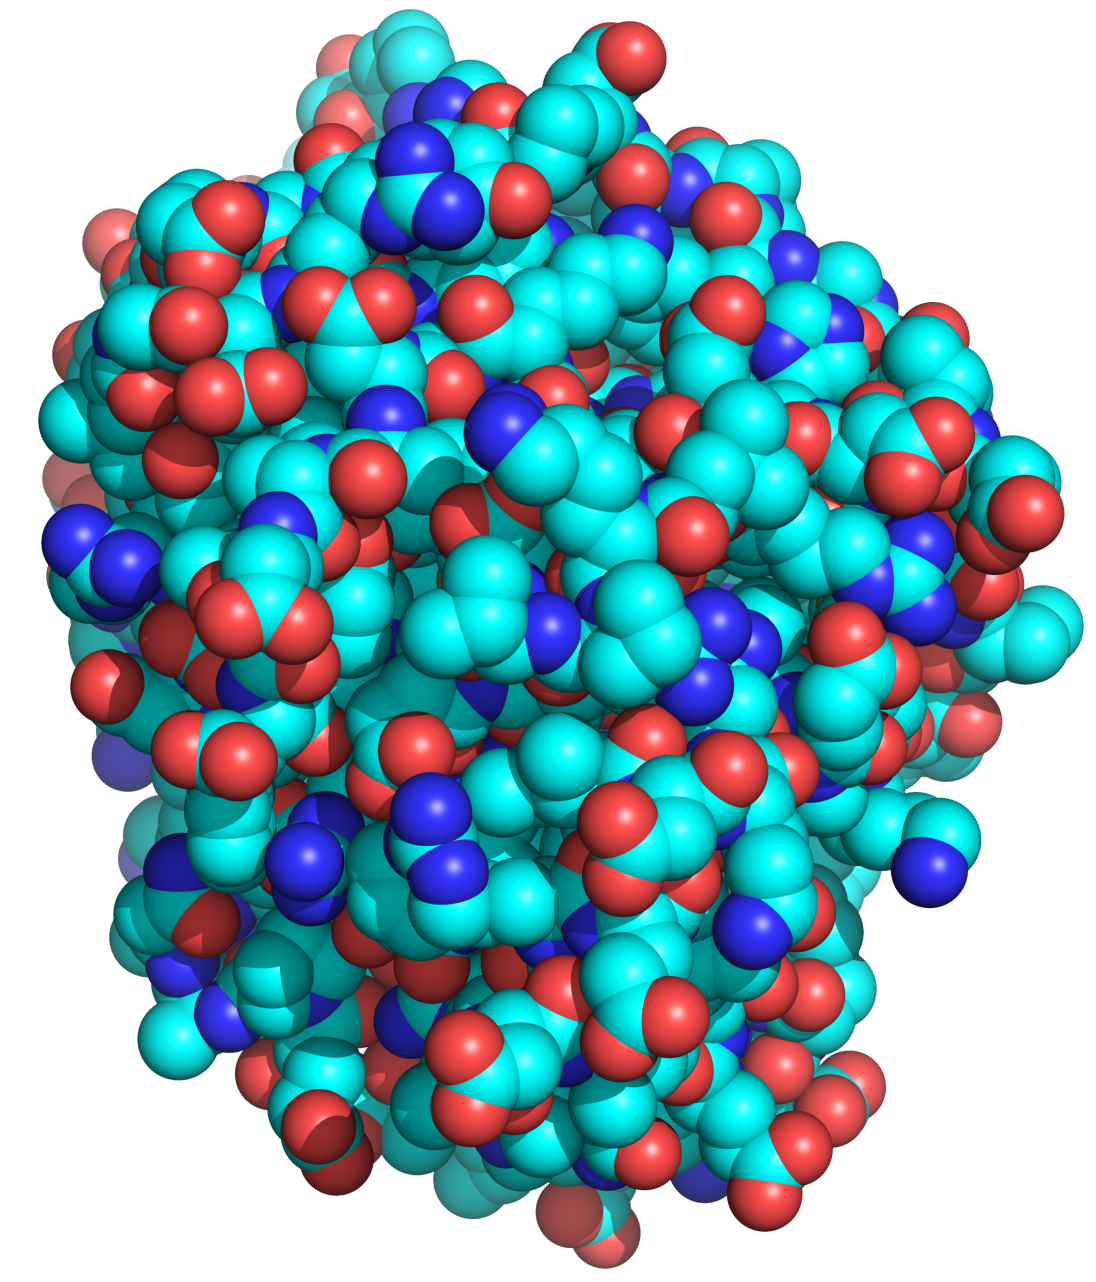
\includegraphics[width=0.24\textwidth]
{fig/motiv1} &
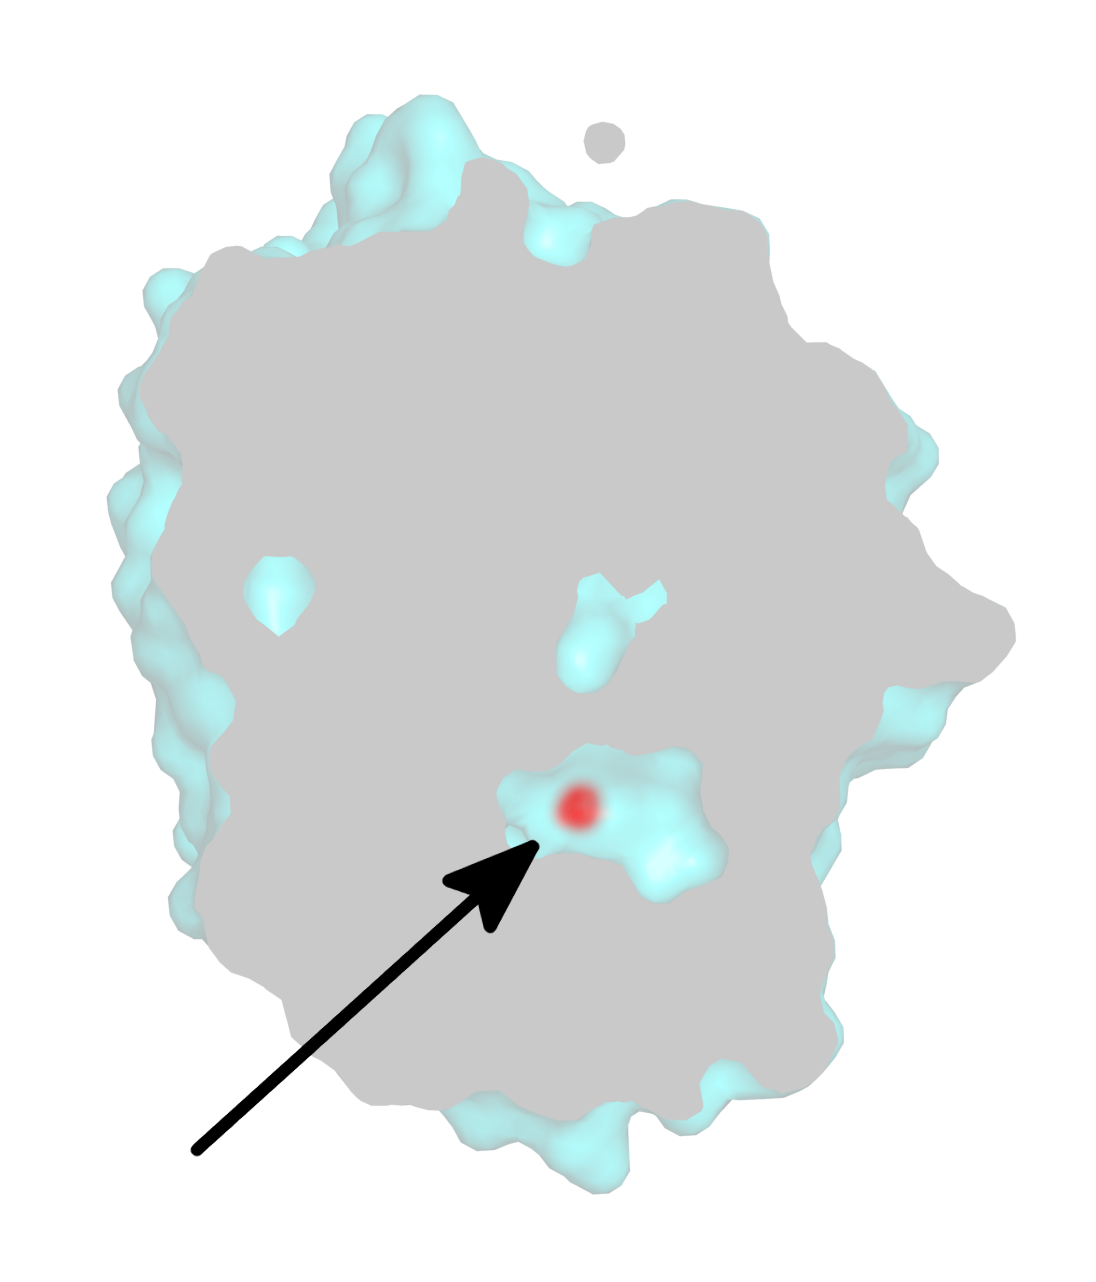
\includegraphics[width=0.25\textwidth]
{fig/motiv2lab} &
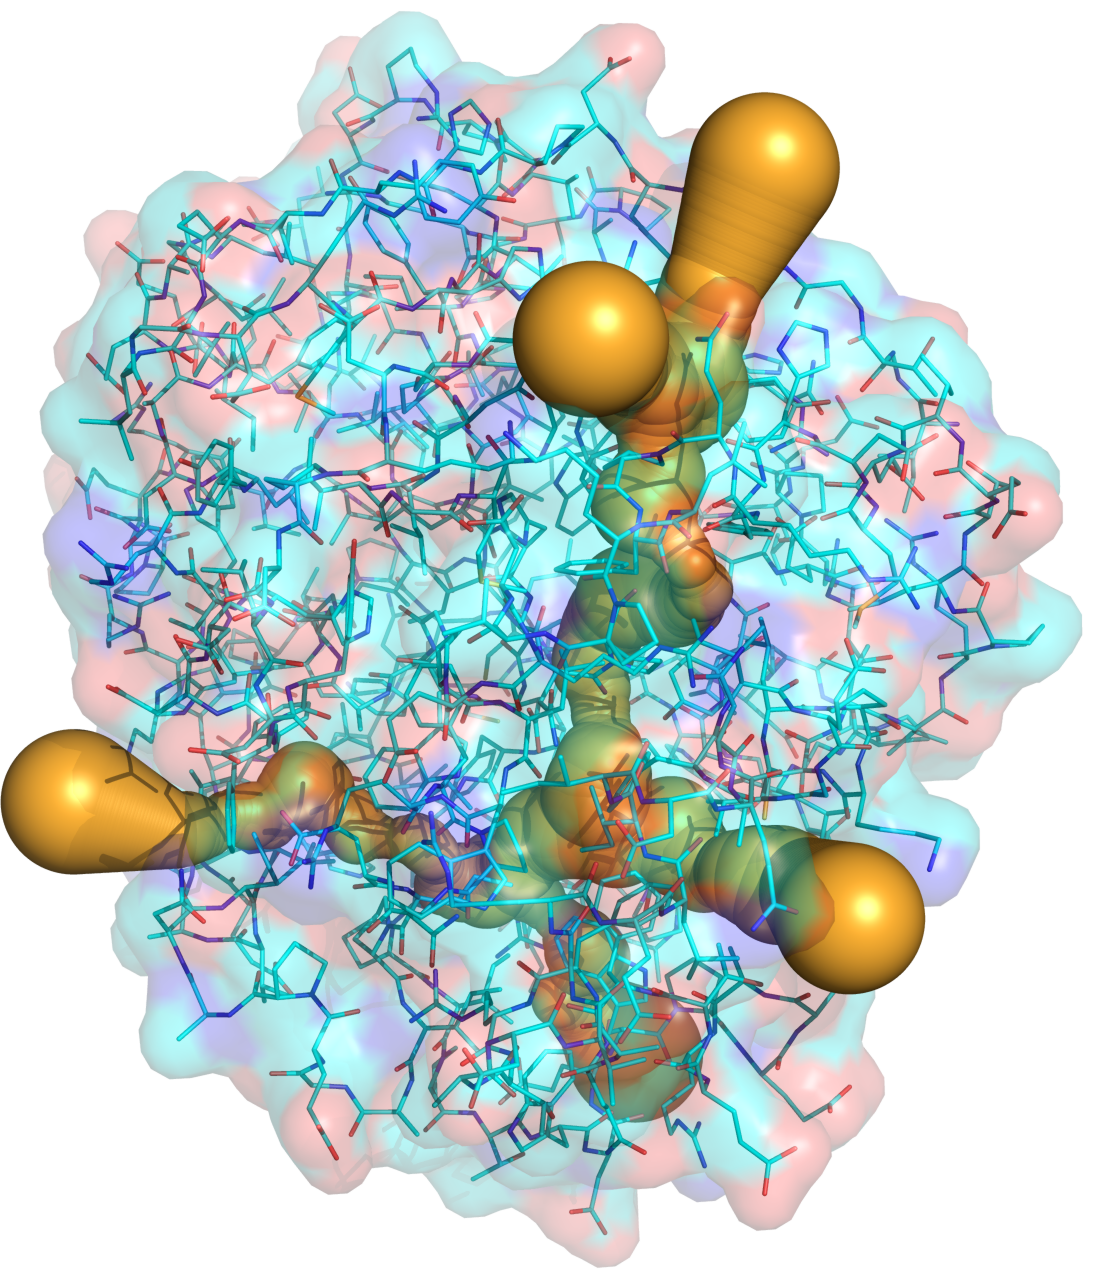
\includegraphics[width=0.24\textwidth]
{fig/motiv3}  \\
Protein  & Active site & Detected tunnels \\ %& Example of a  \\
             &            & (orange)         \\  %& trajectory
\multicolumn{3}{c}{%
\includegraphics[width=0.26\textwidth]
{fig/renderDCP.png}  \hskip 15pt
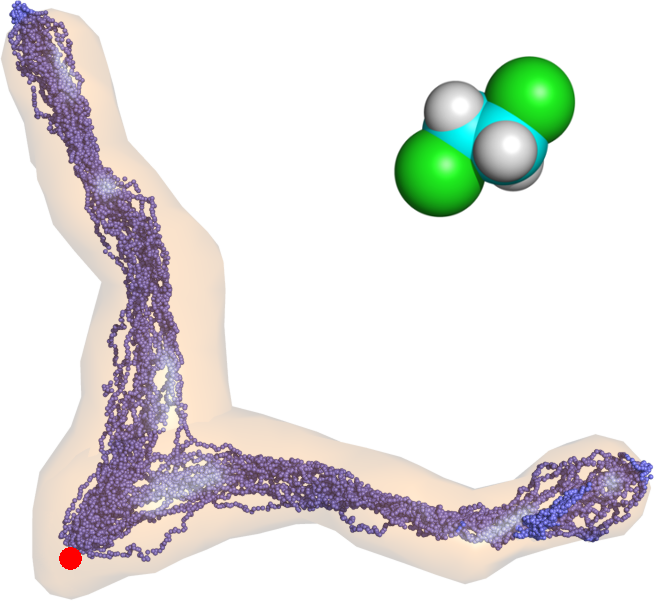
\includegraphics[width=0.24\textwidth]
{fig/render37t.png}} \\ 
\end{tabular}
}
\caption{\label{fig::motiv}
    \small
    Tunnels in the Haloalkane dehalogenase protein with possible trajectories of 1-Chlorpropane ligand (bottom left) and 1,2-Dichloroethane (bottom right).
}
\end{figure}

To solve this problem, other computational methods have to be explored.
In our approach, we are aiming to overcome this by incorporating the path planning methods, which can take into account the actual shape of the ligand.
This necessarily requires to consider also the conformational changes of the ligand, i.e., the changes in the mutual positions of the ligand atoms.
Such ligand is denoted as a \textit{flexible ligand}.

The analysis of the traversability of tunnels by such flexible ligands can be formulated as a motion planning problem and solved by sampling-based planners.
The sampling-based planners randomly sample the configuration space of the robot (ligand) and connect the collision-free samples into a graph structure (roadmap).
Rapidly Exploring Random Tree (RRT)~\cite{lavalleRRT} is one of the most used sampling-based planners. 
Besides many applications in robotics, the sampling-based planners have been already used in biochemistry as well, e.g., to study loop motions~\cite{cortes2004geometric}, to identify binding sites~\cite{bayazit2001ligand}, for exit pathway detection~\cite{cortes2010simulating,cortes2005path}, for tunnel detection~\cite{vonasek2017tunnel}, and especially for protein folding~\cite{raveh2009rapid,amato2002using}. %novinskaya2015improving

In this paper, the novelty lies in modifying the RRT planner to find trajectories for non-spherical flexible ligands inside protein tunnels.
The tunnel is represented by a set of consecutive spheres surrounding the tunnel centerline, a common output of the Voronoi-based tunnel detection tools.
Random samples are then generated only around such detected tunnel, instead of the whole configuration space inside the protein.
The most critical parts for the planning are the narrow sites of the tunnel, where the ligand often has to change its orientation or shape to be able to pass through.
To enable the movement of the ligand in these narrow parts, the free-space inside the tunnel is dilated by shrinking the atom radii, similarly to, e.g., Hsu et al.~\cite{hsu06multilevel}.  %cortes2005path removed as it is not clear it they really rescale
The flexibility of the ligand is then achieved by changing all or a subset of ligand dihedral angles.

Finding trajectories only along a given tunnel is faster than computing all possible exit paths, due to the decreased volume of the searched configuration space.
Another advantage of our method, in comparison with the existing approaches, is that we enable the users to trace the ligand path leading from the outer solvent towards the protein active site.

The proposed method was tested by the biochemists who compared the results with already known trajectories of ligands, determined by their traditionally used approaches and workflows.
We also performed the comparison of the performance of our method with the existing ones and we present our results.
%In the following section, we first mention several approaches and methods related to our solution and then describe the proposed method in detail.


\subsection*{Related Work}

Transportation of ligands into the protein active site can be directly evaluated using molecular dynamics (MD) simulations, where both the protein and ligand are flexible.
However, MD simulations are considerably computational demanding~\cite{kingsley2014including} and they have to be prepared
for a particular ligand/protein pair, which is not practical for testing a large number of different ligands interacting with the protein.
Therefore, computational approaches considering only geometry of the ligand and protein are still preferable due to their high speed.

The widely used approaches to evaluate the ligand traversability rely on the tunnel detection.
Most of the available tools for tunnel detection are based on Voronoi diagrams~\cite{yaffe2008,caver3,sehnal2013mole}.
Tunnels are represented as a sequence of spheres and characterized by their bottleneck, length, curvature, and the list of surrounding residues, whose physico-chemical properties are crucial for assessing of the feasibility of the protein-ligand interactions.
The tunnels are detected either on a single conformation of the protein, or, on a set of protein conformations, generated by MD simulations.
Computationally less demanding approaches for generating possible protein conformations are based on constrained geometric simulations, such as
ROCK~\cite{lei2004sampling}, FRODA~\cite{wells2005constrained}, and tCONCOORD~\cite{seeliger2007geometry}.
Examples of utilization of protein tunnels can be found in the recently published state-of-the-art report about the analysis and visualization of biomolecular cavities~\cite{Krone_2016}.

The main disadvantage of Voronoi diagram-based tunnel detection methods is that the shape of the ligand is not taken into account during the tunnel detection.
Therefore, it is not easy to estimate if (and how) a non-spherical ligand can traverse the tunnel.
The ligand flexibility cannot be principally considered by Voronoi-based approaches and other techniques have to be adopted to solve this problem.

Another possible approach to the detection of the void space inside proteins has been published by Masood et al.~\cite{masood2015chexvis}.
Their CHEXVIS tool utilizes the alpha complexes to detect channels and pores inside proteins.
This alternative method produces tunnels in the same form as the Voronoi-based approach, i.e., as a set of intersecting spheres.
Thus, it also does not take into account the ligand shape. 

The traversability of a tunnel by a flexible ligand of an arbitrary shape can be formulated as a motion planning problem and solved using the sampling-based motion planners.
These planners can cope with objects (robots) with many Degrees of Freedom (DOF) and they can also consider objects of an arbitrary shape.
Two widely used planners are the Probabilistic Roadmaps (PRM)~\cite{kavrakiForPP} and the Rapidly Exploring Random Tree (RRT)~\cite{lavalleRRT}.
The well-known issue of the sampling-based planners is the narrow passage problem.
The narrow passage is a small region in the configuration space, whose removal changes the connectivity of the space.
Due to its low volume, the probability of sampling the narrow passage is low.
Consequently, many iterations are needed in order to put enough samples into the passages, which increases the computational time.
The PRM-based planners can cope with the narrow passage problem by increasing the probability of sampling in difficult regions, e.g., by sampling along the medial axis~\cite{wilmarthMAPRM}.
In~\cite{bergWIG}, the workspace is represented by a grid in which the difficult regions are identified using watershed labeling.
The regions can be estimated online, e.g., based on the number of collision-free samples around a given configuration~\cite{overmarsGauss,hsuBridge} or even identified by a human operator~\cite{denny2018general}. 

In the case of RRT-based planners, increasing the probability of sampling in difficult regions does not need to bring any advantage
if the growth of the tree is blocked by the obstacles.
To prevent this blocking, DD-RRT~\cite{yershovaDDRRT} limits the selection of nodes for the expansion to a small ball. 
The radius of this ball is set to infinity for new nodes, and decreases to a predefined radius if the node cannot be successfully expanded.
An automatic adaptation of this radius was proposed in the ADD-RRT~\cite{jailletADRRT}.
To attract the tree towards a given region, random samples have to be generated there only if the tree can expand to this region.
In~\cite{kardossRRTKK}, the probability of sampling is increased in several waypoints close to the narrow passages, but without specifying how to find these waypoints.
The generalization of~\cite{kardossRRTKK} is the guided sampling, where a sequence of waypoints (a guiding path) is used to generate samples in the configuration space.
The guiding path can be computed in the workspace~\cite{vonasek2009rrt}, or iteratively refined in the configuration space based on the solution of a relaxed version of the problem~\cite{bayazitIRC}.

In the Retraction-based RRT~\cite{zhangRetraction}, the tree is retracted along the boundary of the obstacles in the configuration space.
The Selective Retraction-based RRT~\cite{lee2012srrrt} avoids the expensive growth in the open areas of the configuration space and focuses the retractions only on the narrow passages.
The Obstacle-based RRT~\cite{amatoOBRRT} utilizes several expansion procedures based on, e.g., random vectors, obstacle vectors, or medial axis.
In MARRT~\cite{denny2014marrt}, newly generated samples are pushed towards the medial axis.

In~\cite{singhLIG}, the PRM planner was applied in the ligand binding task.
The roadmap is constructed in the configuration space and each node and edge are evaluated also using the potential energy.
The high-energy configurations are discarded, while the low-energy configurations (and their vicinity) are sampled densely.
This allows to find energy-efficient paths towards the desired binding sites. 
By detecting the configurations near the protein surface that have the lowest energy and oversampling these regions, the
tool~\cite{singhLIG} can also predict the binding sites.

A robotic-based approach was applied for exploring conformational landscape of cyclic peptides in~\cite{jusot2018exhaustive}.
Similarly to our work and~\cite{cortes2010simulating}, the peptides are modeled as a kinematic chain.
In the case of cyclic peptides, the kinematic chain is closed, which makes the sampling of conformational changes more difficult.
Therefore, the conformations are sampled in two phases.
First, first the conformations are sampled using only the dihedral angles and the inverse kinematics is used to enforce the loop closure.
This results in a set of backbone conformations. 
In the second phase, these backbone conformations are further refined considering also the side chains.

The most relevant method to our research is the MoMa-LigPath tool~\cite{cortes2010simulating} that computes exit pathways
for small flexible molecules.
The molecules are modeled as a kinematic chain allowing to consider also the conformational changes.
The pathways are computed using the robotic motion planning, namely using the RRT-ML planner~\cite{cortes2007mlrrt}.
RRT-ML expands the tree primarily using those DOFs, that are essential for achieving the motion of the ligand (i.e., rotation
and translation) and it employs other DOFs (i.e., those that are responsible for conformational changes) if they hinder the growth of the tree.
To further increase probability of finding a solution, radii of the atoms are scaled down slightly in~\cite{cortes2010simulating}, the default
value is 0.7 of the original radii.
This scaling-down effectively increases the volume of the narrow passages in the configuration space, which is often used
in the motion planning literature~\cite{bayazitIRC,vonasek2018motion,hsu06multilevel}.
In the comparison to the methods presented in this paper, the tool~\cite{cortes2010simulating} computes any exit pathway without allowing the user to focus the search to a selected tunnel only.


\subsection*{Contributions}

The main novelty of our proposed approach lies in the utilization of the sampling-based motion planning to compute trajectories of flexible ligands inside protein tunnels.
The input of our approach is formed by a set of tunnels computed using Voronoi diagrams, defining our configuration space.
The method then computes feasible trajectories for a given ligand along these tunnels. 
The trajectories can be computed both from the surface of the protein to the active sice or vice versa.

%The tunnels are detected on selected protein conformations, resulting, e.g., from MD simulations or from a tool providing the protein conformation sampling~\cite{lei2004sampling,wells2005constrained,seeliger2007geometry}.

In contrast to the method proposed by Cort{\'e}s et al.~\cite{cortes2010simulating}, which searches for any exit pathway from the protein, we localize the searching into selected tunnels and compute the trajectories only along each tunnel separately.
This leads to significant speed-up of the calculation and allows the biochemists to further evaluate the feasibility of the detected tunnels and filter out the irrelevant ones, before performing the costly in-vitro experiments in lab.

Computing the trajectories along a single tunnel brings several advantages from the motion planning point of view as well.
The random samples are not generated in the whole configuration space, but only around the tunnel in a user-defined distance. 
This helps to cope with the narrow passage problem.
By selecting a tunnel to be analyzed, the users help the planner to focus only on a subset of the whole configuration
space. 
Consequently, the volume of the configuration space to be searched is decreased, while the relative volume of the narrow passages is increased.
This user-defined focus has been shown beneficial in the sampling-based planning~\cite{denny2018general}.

It has been observed that tunnels detected in protein conformations without ligands (provided by MD simulations without ligands or by
protein conformation sampling) are rather narrow. 
However, MD simulations of proteins with ligands have shown that the tunnels can move, merge and adapt to the shape of the passing ligand and vice versa.
In consequence, even very narrow tunnels, being too small for the passage of a given ligand-approximating sphere, can potentially serve as the transportation path for the ligand.
Therefore, also the existing Voronoi-based methods enable the user to decrease the size of the approximating sphere which simulates the shrinking of the ligand size.
In our solution, we simulate this by shrinking the atom radii of the ligand, which is used also by~\cite{cortes2010simulating,guieysse2008structure}.

%MD simulations of ligands passing through proteins show that the ligands can be highly flexible.
%All possible conformations of a ligand are determined by the torsion and dihedral angles between its atoms, but the low-energy conformations are preferred.
%Therefore, the ligand flexibility can be modeled using only a predefined set of low-energy conformations.
%By using the set of predefined conformations, it is not necessary to model the additional degrees of freedom, so 
%the dimension of the configuration space is not increased as in~\cite{cortes2010simulating}.
%



\section*{Methods}

%\subsection*{Preliminaries}

Proteins and ligands are represented by the hard sphere model, where each atom is represented by a sphere and whose radius 
is the van der Waals radius.
The protein is considered as static, i.e., only the 3D positions of the atoms (and their radii) are representing the protein.
The ligands are considered as flexible, their are modeled as an articulated kinematic chain with $m$ degrees of freedom.
These degrees of freedom are determined by the rotatable bonds of the ligand which is described by the PDBQT~\cite{pdbqt} format.

A configuration $q=(x,y,z,r_x,r_y,r_z, \alpha_1,\ldots,\alpha_m)$ of the ligand describes its 3D 
position $(x,y,z)$, 3D rotation $(r_x,r_y,r_z)$ and $m$ internal degrees of freedom $\alpha_i$ modeling  the rotatable bonds.
All configurations form the configuration space $\C$.
The configurations, where the ligand does not collide with the protein, form the subset $\CF \subseteq \C$.


A protein tunnel is described by a sequence of $n_t$ collision-free spheres $T=( (c_i, r_i) )$, $i=1,\ldots,n_t$, 
where $c_i \in$ $\mathbb{R}^3$ is the center and $r_i > 0$ is the radius of the $i$-th spehere.
The tunnels can be computed using any existing tool, e.g., CAVER 3.0~\cite{caver3}, or CHEXVIS~\cite{masood2015chexvis}.

Let $a_i(q) \in \R^3$ is the 3D position of the $i$-th atom of the ligand determined by the configuration $q \in \C$.
These atom positions are used to determine the distance between two  configururations $q,q' \in \C$ of the ligand:

\begin{equation}
\label{eq::distance}
\dist(q,q') = \sum_{i=0}^{n_l} \distt( a_i(q),a_i(q') )
\end{equation}

\noindent
where $n_l$ is the number of atoms of the ligand, and $\distt$ is the 3D Euclidean metric.
By computing the distance $\dist$ using the atom positions, the flexbility of the ligand is taken into account.

Collision detection between the atoms of the ligand and the atoms of the protein is used to determine collision-free samples.
Fast collision detection can be realized using hierarchical methods such as bounding volume hiearchy~\cite{ericson2004real}.
In the case of protein/ligand interactions, it is common to enable little penetration between the ligand's and 
the protein's atoms~\cite{cortes2010simulating}, which can be achieved by a slight decrease
of the atom radii, e.g., to the 80~\% of the original value, which is also considered in this paper.


\subsection*{Computing Ligand's trajectories using Sampling-based Planning}

The task of finding the trajectory of the ligand can be solved by finding a path from the
start configuration $\qstart \in \CF$ towards the goal $\qgoal \in \CF$.
The start and goal configurations are determined by the start and end of the protein tunnel, respectively.

The trajectories of the ligand are found using the RRT principle~\cite{lavalleRRT} that is extended to focus the search towards the selected protein tunnel.
The proposed method is listed in Alg.~\ref{alg::main}.
The algorithm builds the tree $\T$ of collision-free configuration. 
The tree is rooted at the initial configuration $\qstart \in \CF$.
In each iteration, a random sample $\qrand \in \C$ is generated and its nearest neighbor $\qnear \in \T$ 
in the tree $\T$ is found according to the metric $\dist$.
The node $\qnear$ is then expanded.
The algorithm is terminated if the goal $\qgoal$ is reached to a user-define distance.

The task of the expansion is to find new collision-free configuration $\qnew \in \C$ around $\qnear$ that minimizes the distance
Eq.~\eqref{eq::distance} towards $\qrand$.
The vicinity of $\qnear$ is sampled by $k$ random samples $\qnew'$. 
The translational part of $\qnew'$ is generated from $N(pos(\qnear),\Sigma')$, 
where $pos(\qnear)$ is the translational part of $\qnear$ and $\Sigma'$ is
the $3 \times 3$ diagonal matrix with values $\varepsilon$ on the diagonal, and $\varepsilon$ is the resolution of the planner.
The rotational part of $\qnew'$ is generated from $N(rot(\qnear), \Sigma_r)$, where $\Sigma_r$ is the $3 \times 3$ diagonal
matrix with values $\pi/3$ and the internal degrees of freedom $\alpha_i$ of $\qnew'$ are generated
randomly from $U(-\pi,\pi)$.
Each sample $\qnew'$ is checked for collision and the from the collision-free one samples, the nearest towards $\qrand$ is 
selected, which results in a new configuration $\qnew$.
The resulting configuration is then added to the tree and the node $\qnear$ is marked as the parent of the node $\qnew$.
During the expansion (Alg.~\ref{alg::expand}), the vicinity of $\qnear$ is sampled with $N$ predefined samples.
The samples are tested for collisions and the collision-free samples, that minimize the distance to $\qrand$ are added to the tree.

The crucial part of the RRT-based search is the generation of random samples.
In the classic RRT~\cite{lavalleRRT}, the random samples are generated uniformly from the whole configuration space $\C$.
The uniformly generated samples $\qrand$ supports the quick expansion of the configuration tree $\T$ towards the unexplored
regions of the configuration space.
However, in the case trajectory planning in protein tunnels, the growth of the tree outside the tunnels is not desired.
Instead, the growth of the tree should be contrainted only along the vicinity of the tunnel.

Finding ligand trajectories in the tunnels requires to steer the growth of the tree from the start of the tunnel to its end.
This is achieved by generating the random samples $\qrand$ progresivelly along the tunnel.
Let $1 \le v \le n$ denote the index of a sphere $c_v$ of the tunnel, we denote to this sphere as to the active sphere in the rest of the paper.
The random sample $\qrand$ is generated around  $c_v$ with probability $\gb$; otherwise, it is generated uniformly in $\C$.
To generate the random sampla around the active sphere $c_v$, the 3D position of $\qrand$ is generated from $N(c_i,\Sigma)$, where
$\Sigma$ is the $3\times 3$ diagonal matrix with value $r_v$ on the diagonal.
The rotational part of $\qrand$ is generated uniformly, i.e., $r_x,r_y,r_z \sim U(-\pi,\pi)$ and the internal degrees of 
freedom $\alpha_i=0$, $i=1,\ldots,m$.

At the begining of the algorithm, the active sphere is set to the begining of the tunnel, $v=1$.
After the sucessful expansion, the distance to the center of the active sphere is calculated.
If the tree approaches the active sphere to the predefined distance $\dtg$, new active sphere of the tunnel is determined.
The distance $\distt(c_i, q'), i=v+1,\ldots,n$ between each subsequent sphere and it's nearest node in the tree $q' \in \T$ 
is calculated. 
The sphere with the lowest index $i$ whose distance towards the tree is larger than $\dtg$ is set as the active sphere.
Setting the virtual goal to this successor allows the tree to avoid such parts of the tunnels that are not traversable or reachable by the ligand.
The tree can slightly detour from the tunnel and overcome difficult parts (e.g., the tunnel bottleneck) by finding an alternative trajectory nearby.
Example of the shifting of the active sphere is depicted in Fig.~\ref{fig::active}.

\begin{figure}
\centering
{
\renewcommand{\tabcolsep}{2pt}
\begin{tabular}{cccc}
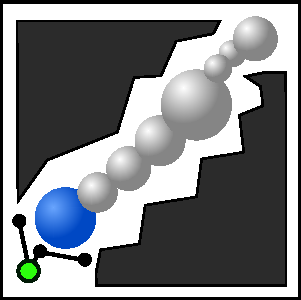
\includegraphics[width=0.23\textwidth]{fig/temporary_goal_nodeA} &
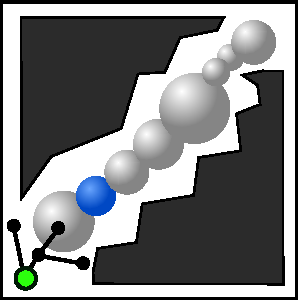
\includegraphics[width=0.23\textwidth]{fig/temporary_goal_nodeB} &
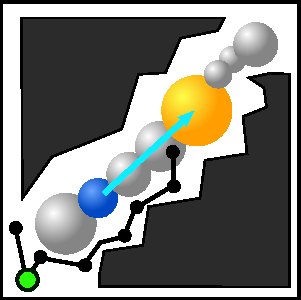
\includegraphics[width=0.23\textwidth]{fig/temporary_goal_nodeC} &
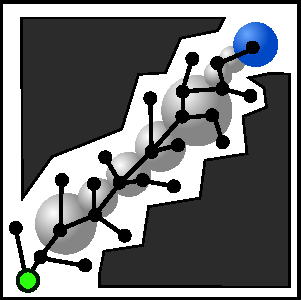
\includegraphics[width=0.23\textwidth]{fig/temporary_goal_nodeD} \\
a & b & c & d \\
\end{tabular}
}
\caption{\label{fig::active}
Example of shifting the active sphere along the tunnel (grey spheres).
The random samples are generated around the active sphere (blue) (a).
The active sphere is moved forward if the tree approaches it (b); the active sphere can be moved even further if
the tree skips several tunnel spheres (c).
The results of the planning method is the configuration tree growing along the tunnel (d).
}
\end{figure}

The parameter $\dtg$ determines how far can the tree detour from the tunnel centerline.
In case of tunnels not having other tunnels in the close vicinity (which is very common), we recommend using the double value of the tunnel average width.
The algorithm terminates after a predefined number of planning trials $\Imax$ or if the tree reaches
the last sphere in the tunnel, i.e., when $v = n$.
%and the rotational part of $\qrand$ is generated using techniques described in~\cite{kuffnerES}.

The nearest-neighbor search required to find $\qnear$ (line~\ref{alg::kdtree} in Alg.~\ref{alg::main}) can be realized
using KD-tree data structure.
After a succesfull expansion by the confiuration $\qnew$, new vector of atom positions $a_i(\qnew)$ is added to the KD-tree.


\def\ccolor{\color{gray}}

\LinesNumbered
\begin{algorithm}[b]
\DontPrintSemicolon
{\small
\setstretch{0.88}
\caption{\label{alg::main}Trajectory planner}
\KwIn{
    tunnel $T=( (c_i, r_i) )$, $i=1,\ldots,n$, with spheres centers $c_i \in \R^3$ and radii $r_i$,
    initial configuration $\qinit$
}
\KwData{
   distance $\dtg$ to move virtual goal,
   tunnel bias $\gb$
}
\KwOut{
    configuration tree $\T$
}
\hrule
$v = 1$  \tcp*{\ccolor index of the virtual goal}
$iteration = 0$ \tcp*{\ccolor planning iteration}
$\T$.addNode($\qinit$) \tcp*{\ccolor tree is rooted at $\qinit$}
\While{$iteration < \Imax$ {\bf and}  $v < n$}{
    \eIf(\tcp*[f]{\ccolor generate random sample }){$rand() < \gb$}{
        $\qrand$ = random sample around virtual goal $c_v\!\in\!T$ \nllabel{main::s1} \\
    }{
        $\qrand$ = random sample from $\C$ \nllabel{main::s2} \\
    }
    $\qnear$ = nearest node in $\T$ towards $\qrand$ \nllabel{alg::kdtree} \tcp*{\ccolor using metric $\dist$ from Eq.~\eqref{eq::distance}}
    expand($\T, \qnear,\qrand$) \tcp*{\ccolor Alg.~\ref{alg::expand}}
    \For(\tcp*[f]{\ccolor find last reached sphere}){$i=n,n-2,\ldots,v$}{ \nllabel{alg::main:a} 
        $q'$=$\T$.nearestNode($c_i$) \tcp*{\ccolor nearest node to sphere $c_i$ using $\distt$ metric}
        \If(\tcp*[f]{\ccolor is sphere $c_i$ reached by the tree?}){$\distt(c_i,q') < \dtg $}{
            $v = i+1$; \tcp*{\ccolor new virtual goal found} 
            {\bf  break}
        }
    } \nllabel{alg::main:b}
    \If(\tcp*[f]{\ccolor the tree reaches the  last tunnel's sphere}){$v=n+1$}{
        return $\T$.findPath($\qinit,\qnew$) \tcp*{\ccolor resulting path}
    }
    $iteration = iteration+1$\;
}
\return failure \tcp*{\ccolor no path is found from start to goal}
}
\end{algorithm}


\begin{algorithm}[b]
\DontPrintSemicolon
{\small
\setstretch{0.88}
\caption{\label{alg::expand}expand}
\KwIn{
   tree $\T$,
   configuration $\qnear$ to be expanded,
   random configuration $\qrand$
}
\KwData{
   number of trials $k$
}
\hrule

$\qnew = \emptyset$ \tcp*{\ccolor empty configuration \nllabel{alg::expa}}
\For{$i = 1,\ldots,k$}{
    $q=\qnear$ \\
    $q.position$ = random 3D position around $\qnear$ \\
    $q.rotation$ = random 3D rotation \\
    \If{isCollisionFree($q$)}{
        \If{$\qnew = \emptyset$ {\bf or} $\dist(q, \qrand) < \dist(\qnew,\qrand)$}{ \nllabel{alg::expand:a}
            $\qnew = q$ \tcp*{\ccolor new candidate configuration}
        }
    } 
}
\nllabel{alg::expb}
\If(\tcp*[f]{\ccolor expands the tree by $\qnew$}){$\qnew \ne \emptyset$} {
    $\T$.addNode($\qnew$) \\
    $\T$.addEdge($\qnear,\qnew$) \\
}
}
\end{algorithm}


\section*{Results and Discussion}
\subsection*{Experimental Verification}

The proposed algorithm was verified on a set of various proteins and ligands. 
In each protein, tunnels for spherical probe 1.0~\AA were found using CAVER 3.0~\cite{caver3}.
The default settings of CAVER 3.0 were used and the tunnels were ranked according to the default CAVER 3.0 ranking system.
The analysis was performed in the first two tunnels.

The PDB IDs of the tested proteins are:
1AKD (3208 atoms),
1BL8 (2823 atoms),
1MXTA (8343 atoms),
1PV7 (6581 atoms),
1ZNJ (2382 atoms),
2ACE (4144 atoms),
2BG9 (14928 atoms),
2OAR (4762 atoms),
5JQH (7601 atoms).

A set of small ligands were tested:

The ligands:
Dichloropropanol (DCP) (12 atoms, 2 DOFS),
1-chloropropane (m003) (4 atoms, 1 DOF),
1,2-Dichloroethane (m037t) (4 atoms, 1 DOF),
3-chloropropene (m207) (4 atoms, 1DOF),
1,3-Dichloropropane (m038t) (5 atoms, 2 DOFs),
(R)-bromobutane (m062r) (5 atoms, 1 DOF),
m113 - epichlorohydrin (m113) (5 atoms, 1 DOF),
1,3-(E)-dichloropropene (m210e) (5 atoms, 1 DOF),
Trichloropropane (m080) (6 atoms, 2 DOFs),
2-chloroethylvynilether (m112) (6 atoms, 3 DOFs),
2-bromoacetonitrile (m133) (4 atoms, 0 DOFs),
4-bromobutyronitrile (m141) (6 atoms, 2 DOFs).


%    ---- names of ligands from Ondra ----
%m037t (1,2-Dichloroethane), m038t (1,3-Dichloropropane), m056 (2-Chlorobutane), and m080 (Trichloropropane).
%m003 - 1-chloropropane
%m207 - 3-chloropropene
%m62r - (R)-bromobutane
%m113 - epichlorohydrin
%m210e - 1,3-(E)-dichloropropene
%m112 - 2-chloroethylvynilether
%m133 - 2-bromoacetonitrile
%m141 - 4-bromobutyronitrile
%DCP.pdb, Dichloropropanol
%m037t.pdb, 1,2-Dichloroethane
%m038t.pdb, 1,3-Dichloropropane
%m040.pdb, 1,5-Dichloropentane
%m056.pdb, 2-Chlorobutane
%m080.pdb, Trichloropropane

The proposed method was compared to the MoMa-LigPath (MMLP) tool~\cite{cortes2010simulating}.
Default settings was used in the case of MMLP. The most important parameter was scale-down factor of the Van der Waals radii, which is 
0.7. 
We, therefore, used the same scaling factor in our method.

For each combination of protein, tunnel and ligand, 50 initial configurations were found at the vicinity of 3~\AA around the active site.
These configurations were then used by both tested methods.
The proposed planner was terminated if it reaches the last sphere of the tunnel to the distance 2~\AA or less.
The terminate condition of the MMLP planner cannot be set by the user; instead, MMLP terminates if it finds exit pathways that leads far away from the protein.



%\subsubsection*{Analysis of MD simulation}


\subsection*{Discussion and Utilization of the Results}
The presented work is motivated by the current needs of biochemists who need to analyze the traversability of selected ligands through selected protein tunnels.
Due to the low bottleneck of tunnels, it is often required to shrink the atomic radii of the ligand, as utilized also in other existing tools.
Finding trajectories for the scaled-down ligands enables to solve the problem with narrow passages, but it can be questionable how biochemically relevant such trajectories~are.

Determination of the proper scaling-down factor requires long-term testing of many exemplary simulations and needs to be performed by the biochemists. 
Therefore, it is beyond the scope of this paper, which focuses namely on the algorithmic part of the problem.
The scales used at the trajectory points can provide the biochemists with new knowledge about the ligand behavior, which was impossible to get using the Voronoi-based approaches.
Judging the accessibility of the active site by a ligand based only on the traversability rates may be problematic if the ligand is scaled down too much.
The visualization of the computed trajectories can show those parts of the tunnel where the ligand had to be scaled-down significantly (red parts of trajectories in Fig.~\ref{fig::dcp}), and parts where the ligand could be enlarged again (green parts in Fig.~\ref{fig::dcp}).

According to the results of the motion planning, the DCP ligand needs to shrink down to approximately 75~\% of its size, but only at one part of the tunnel (Fig.~\ref{fig::dcp}, point B). 
Beyond this point, the ligand can move at larger scales again.
As both the protein and ligand mutually influence each other, it is possible that even such a narrow part of the tunnel is traversable.
This was observed in a separate MD simulation of the DCP ligand in the 4E46 protein, which revealed that DCP can pass the main tunnel~\cite{marques2017catalytic}. 
The necessity to scaled-down even more than 0.8, which is a value used by other tools~\cite{cortes2010simulating}, was
shown also in the second experiment, where the trajectory for the inhibitor of the 4L2L protein required scaling down to 0.5 or 0.6.


\begin{figure}
\centering
\vskip -5pt
\includegraphics[width=0.8\textwidth]{fig/dcp-image1Label}\\
\vspace{-5pt}
\caption{\label{fig::dcp}
    \small
Visualization of trajectories for the ligand DCP in the two examined tunnels.  
The color of the trajectories corresponds to the scale, that was needed to pass the given part of the tunnel.
The ligand can enter the first tunnel with a high scale (almost 1=100~\%) (A), but then it has to be scaled-down (to $\sim75$~\%) to pass the
next part of the tunnel (B). After this narrow passage, the tunnel is larger again and the ligand can traverse to the narrow passage with
scale $>75$~\% (C).
The second tunnel can also be entered with the high scale (green), but then the narrow part is traversable only with a low scale ($\sim50$~\%) (D). 
For the visualization purposes, even more scale-down to 0.3=30~\% was allowed (E) to see how the ligand passed the tunnel.
The ligand can reach the active site only at a very low scale ($\sim0.4=40$~\%) using the side tunnel.
}
\end{figure}

\subsection*{Conclusion}
We presented a novel modification of the RRT planner to compute trajectories of ligands inside selected protein tunnels.
The ligand shape is taken into account and the ligand flexibility is modeled using a predefined set of its conformations.
The ligand conformations are prepared using the Rosetta tool, ranked by their energy and only low-energy conformations are used in the planning.
To simulate the real behavior of ligand passing through the tunnel, we enable scaling down the atomic radii of the ligand up to a certain predefined factor.
The planner generates the random samples only along a tunnel computed by the Voronoi diagram, and it attempts to expand the configuration
tree using all ligand conformations. 
The expansion prefers atoms with a higher scale, which ensures that the ligand shrinks down only if necessary, i.e., when traversing the narrow parts of the tunnel.

%%%%%%%%%%%%%%%%%%%%%%%%%%%%%%%%%%%%%%%%%%%%%%
%%                                          %%
%% Backmatter begins here                   %%
%%                                          %%
%%%%%%%%%%%%%%%%%%%%%%%%%%%%%%%%%%%%%%%%%%%%%%

\begin{backmatter}

\section*{Competing interests}
  The authors declare that they have no competing interests.

\section*{Author's contributions}
    Text for this section \ldots

\section*{Acknowledgements}
The presented work has been supported by the Czech Science Foundation (GA{\v C}R) under research project No. 17-07690S.
Computational resources were provided by the CESNET and CERIT Scientific Cloud
(grant nos. LM2015042 and LM2015085) and grant of the Ministry of Education of
the Czech Republic ESFRI Czech National Infrastructure for Biological Data (no.
LM2015047). OV is the recipient of a Ph.D. Talent award provided by Brno City Municipality.


%%%%%%%%%%%%%%%%%%%%%%%%%%%%%%%%%%%%%%%%%%%%%%%%%%%%%%%%%%%%%
%%                  The Bibliography                       %%
%%                                                         %%
%%  Bmc_mathpys.bst  will be used to                       %%
%%  create a .BBL file for submission.                     %%
%%  After submission of the .TEX file,                     %%
%%  you will be prompted to submit your .BBL file.         %%
%%                                                         %%
%%                                                         %%
%%  Note that the displayed Bibliography will not          %%
%%  necessarily be rendered by Latex exactly as specified  %%
%%  in the online Instructions for Authors.                %%
%%                                                         %%
%%%%%%%%%%%%%%%%%%%%%%%%%%%%%%%%%%%%%%%%%%%%%%%%%%%%%%%%%%%%%

% if your bibliography is in bibtex format, use those commands:
\bibliographystyle{bmc-mathphys} % Style BST file (bmc-mathphys, vancouver, spbasic).
\bibliography{paper}      % Bibliography file (usually '*.bib' )
% for author-year bibliography (bmc-mathphys or spbasic)
% a) write to bib file (bmc-mathphys only)
% @settings{label, options="nameyear"}
% b) uncomment next line
%\nocite{label}

% or include bibliography directly:
% \begin{thebibliography}
% \bibitem{b1}
% \end{thebibliography}

%%%%%%%%%%%%%%%%%%%%%%%%%%%%%%%%%%%
%%                               %%
%% Figures                       %%
%%                               %%
%% NB: this is for captions and  %%
%% Titles. All graphics must be  %%
%% submitted separately and NOT  %%
%% included in the Tex document  %%
%%                               %%
%%%%%%%%%%%%%%%%%%%%%%%%%%%%%%%%%%%

%%
%% Do not use \listoffigures as most will included as separate files

\section*{Figures}
%  \begin{figure}[h!]
%  \caption{\csentence{Sample figure title.}
%      A short description of the figure content
%      should go here.}
%      \end{figure}

%\begin{figure}[h!]
%  \caption{\csentence{Sample figure title.}
%      Figure legend text.}
%      \end{figure}

%%%%%%%%%%%%%%%%%%%%%%%%%%%%%%%%%%%
%%                               %%
%% Tables                        %%
%%                               %%
%%%%%%%%%%%%%%%%%%%%%%%%%%%%%%%%%%%

%% Use of \listoftables is discouraged.
%%
%\section*{Tables}
%\begin{table}[h!]
%\caption{Sample table title. This is where the description of the table should go.}
%      \begin{tabular}{cccc}
%        \hline
%           & B1  &B2   & B3\\ \hline
%        A1 & 0.1 & 0.2 & 0.3\\
%        A2 & ... & ..  & .\\
%        A3 & ..  & .   & .\\ \hline
%      \end{tabular}
%\end{table}

%%%%%%%%%%%%%%%%%%%%%%%%%%%%%%%%%%%
%%                               %%
%% Additional Files              %%
%%                               %%
%%%%%%%%%%%%%%%%%%%%%%%%%%%%%%%%%%%

%\section*{Additional Files}
%  \subsection*{Additional file 1 --- Sample additional file title}
%    Additional file descriptions text (including details of how to
%    view the file, if it is in a non-standard format or the file extension).  This might
%    refer to a multi-page table or a figure.

%  \subsection*{Additional file 2 --- Sample additional file title}
%    Additional file descriptions text.


\end{backmatter}
\end{document}



% text from old paper related to old experiments

The MD simulation was computed using AMBER~12 (details about the used MD simulations of DhaAwt/4E46 are described in~\cite{marques2017catalytic}).
The tunnels were detected in 100 consecutive frames of MD simulation in the part where the protein was already stabilized.
The tunnels for the probe 0.9~\AA\ towards the active site defined by residues 38 (Asparagine), 102 (Histidine), and 103 (Aspartic Acid) were
computed using the CAVER 3.0~\cite{caver3} tool.
In most of the frames, two tunnels were detected.
The average bottleneck sizes of these tunnels were $1.48$~\AA\ and $1.2$~\AA\ for the main and side tunnel, respectively.

Models  of the ligands in Mol2 formats were converted to the param files~\cite{meiler2006rosettaligand}, containing the topology, rotatable bonds, atom types, and partial charges. 

The methods \RA\ and \RB\ differ in the expansion step (lines \ref{alg::expa}--\ref{alg::expb} in Alg.~\ref{alg::expand}).
In these lines, the \RB\ method employs the retraction step in order to find a new collision-free configuration $\qnew$ that approaches $\qrand$.
The retraction step is realized by sampling the vicinity of the configuration $\qnear$ in the distance $0.05$~\AA\ using 20 samples.
A collision-free sample that maximally approaches $\qrand$ is selected and added to the tree, and the retraction continues from this sample.
The retraction step is repeated 5 times.
The \RB\ method can therefore expand the tree by at most 5 new nodes per ligand conformation, while \RA\ extends the tree only by one new node.
The larger number of nodes in \RB\ method is not problematic, as the KD-trees were used for the nearest-neighbor search and the time to solve these queries is significantly smaller than the collision detection.
The parameters of the methods were selected in such a way that the number of collision detection queries in each expansion step is the same.
For each conformation and tested scale, the \RA\ method checks $m=100$ candidate configurations for collision, and \RB\ checks $5 \times 20$ configurations for collision.
Other parameters of the \RB\ planner were the same as for \RA.
The planning was terminated after $\Imax$ iterations or if the tree approached the active site to the distance less than 2~\AA\ (i.e., the 
geometric center of the ligand was closer than 2~\AA\ from the active site).

The performance of the methods is evaluated using the traversability rate, which is the percentage of frames of the protein dynamics that are traversable by the tested ligand.
This distance is measured as the 3D distance between the geometric center of the ligand and the position of the active site.



\subsubsection*{Analysis of Protein Conformations}
The task of the second analysis was to find the trajectory for the ligand 4-(4-benzylphenyl)-1,3-thiazol-2-amine into the active
site of A4 hydrolase (PDB ID 4L2L, 9666 atoms).
The tCONCOORD tool~\cite{seeliger2007geometry} was used to generate 1000 conformations of the protein 4L2L.
The initial PDB structure was minimized by GROMACS 4.0.7 using the input parameters recommended on the example page of tCONCOORD~\cite{tconcoord}.
The protein conformations were generated using the default settings for tCONCOORD in the PERT mode. % which only perturbs the starting configuration of atoms instead 
The tunnels leading to the active site defined by residues 134 (Alanine) and 311 (Phenylalanine) were computed by CAVER 3.0, using the probe 0.9~\AA.
All 1000 conformations contained at least 5 tunnels. % more than 900 conformations contained 9 tunnels.
The ordering of the detected tunnels slightly differs in different conformations.
Therefore, the first three widest tunnels were used (with average bottlenecks 1.22~\AA, 1.20~\AA\, and 1.19~\AA\ with the average lengths 22.3~\AA, 25.3~\AA\, and 28.4~\AA, respectively).
20 starting configurations were found at the begining of each tunnel, and 10 trajectories were computed for each starting configuration.
The conformations of the ligand were prepared in the same way as in the previous section.
From the available $|\L|=736$ low-energy conformations, 100 were selected using the `S' strategy.

\begin{table}[bt]
\centering
\caption{\label{tab::4l2l}
    \small
    Traversability rate in 1000 conformations of the protein 4L2L in the first three tunnels.
}
\small
\renewcommand{\tabcolsep}{2pt}
{
\scriptsize
%\input traversability.tex
}
\end{table}

As the tested ligand is a known inhibitor of the protein 4L2L~\cite{marques2017enzyme} we assumed that the ligand can reach the active site.
Due to large size of the ligand (33 atoms), low scale-down factors $smin\in\{0.4,0.5,0.6\}$ were used and
the active site was considered as reached if the distance to the geometric center of the ligand was less than 5~\AA.
All parameters of the \RA\ were set as in the previous experiment, except $\Imax=100\cdot10^3$.
The proposed planner was able to find trajectories even for this large ligand inside the long tunnels, which is
shown by the traversability rates (Tab.~\ref{tab::4l2l}).
Example of the solution is depicted in Fig.~\ref{fig::inhibitor}.



For the DCP ligand, the trajectories were detected in 18~\% of frames for scale and the traversability of this ligand
to the active site was approved by a separate MD simulation~\cite{marques2017catalytic}.
Based on the success rate, also other ligands (e.g., m037t with traversability rate 45~\% at $smin$=0.8) seem to be promising.
However, their binding was not yet approved by dedicated MD simulations.
The planning was realized with 50 conformations of the ligands, but not all of them were used, which is shown in Tab.~\ref{tab::m040c}.

Besides scaling-down the ligand, also the atoms of the protein can be scaled, which is used, e.g., in~\cite{cortes2005path}, where the scale 0.8 is used for both the ligand and protein.
We tested also this option using \RA\ (the column \RD\ in Tab.~\ref{tab::main}).
The results are similar to the results of \RA\ and $smin=0.6$ (except for DCP and m040, which can be a result of randomization).

The proposed \RA\ planner provides higher traversability rate than the RRT-Retraction (\RB).
The distances of the configuration trees (measured using the 3D Euclidean metric) to the active site and the runtimes in each frame
are shown in Fig.~\ref{fig::comparison}.
The runtimes of \RB\ are higher than the runtimes of \RA\ and the standard deviations as well.


\paragraph*{Algorithm and data setup}

The traversability rate is shown in Tab.~\ref{tab::main}. 
Only the traversability of the main tunnel is shown, as no trajectory was found in the side tunnel for most of the tested ligands.
The only exception is the ligand m037t, which was the smallest tested one (consisting of 8 atoms), and therefore it could fit even inside the side tunnel.
The traversability rate is higher for the most scaled-down ligands  and it decreases with the increasing scale.


\begin{figure}
\centering
\vskip -5pt
\includegraphics[width=0.8\textwidth]{fig/4l2l-solution.png}
\caption{\small
    \label{fig::inhibitor}Example of a found trajectory inside the tunnel No. 1 of the 4L2L protein with the final position of the ligand.
}
\end{figure}



